% ============================================================
%  EC2L104 - Introduction to EDA Tools : LTspice Exercise Report
%  Template. Put your plots in a folder named  figs/
%  Missing images automatically show as grey placeholder boxes.
% ============================================================
\documentclass[11pt,a4paper]{article}

\usepackage[margin=2.2cm]{geometry}
\usepackage{graphicx}
\usepackage{booktabs,array,tabularx}
\usepackage{amsmath,amssymb}
\usepackage{siunitx}
\usepackage{float}
\usepackage{caption,subcaption}
\usepackage{xcolor}
\usepackage{fancyhdr}
\usepackage{listings}
\usepackage[most]{tcolorbox}
\usepackage[hidelinks]{hyperref}

\graphicspath{{figs/}{s1/}{s2/}{s3/}{s4/}{s5/}{s6/}{s7/}}
\sisetup{detect-all}

% ---------- header / footer ----------
\pagestyle{fancy}
\fancyhf{}
\lhead{EC2L104 -- Introduction to EDA Tools}
\rhead{LTspice Exercise Report}
\cfoot{\thepage}
\renewcommand{\headrulewidth}{0.4pt}

% ---------- code listing style ----------
\lstset{basicstyle=\ttfamily\footnotesize,breaklines=true,
        frame=single,backgroundcolor=\color{gray!8},columns=fullflexible}

% ---------- reusable boxes ----------
\newtcolorbox{observations}{colback=blue!4,colframe=blue!50!black,
  title=Observations,fonttitle=\bfseries\small,boxrule=0.5pt}
\newtcolorbox{conclusion}{colback=green!5,colframe=green!40!black,
  title=Conclusion,fonttitle=\bfseries\small,boxrule=0.5pt}
\newtcolorbox{physics}{colback=orange!6,colframe=orange!60!black,
  title=Device-physics explanation,fonttitle=\bfseries\small,boxrule=0.5pt}

\newcommand{\todo}[1]{\textcolor{red!70!black}{\textit{[#1]}}}
\newcommand{\blank}[1][3cm]{\rule{0pt}{1em}\rule[-0.3ex]{#1}{0.4pt}}

% \gfx{file}{width}{height-if-missing}
% shows the image if it exists, otherwise a placeholder box
\makeatletter
\newif\iffigfound
\newcommand{\figdirs}{./,figs/,s1/,s2/,s3/,s4/,s5/,s6/,s7/}
\newcommand{\gfx}[3]{%
  \figfoundfalse
  \@for\@figdir:=\figdirs\do{\iffigfound\else
    \IfFileExists{\@figdir#1}{\figfoundtrue\xdef\@figpath{\@figdir#1}}{}\fi}%
  \iffigfound
    \includegraphics[width=#2]{\@figpath}%
  \else
    \fbox{\parbox[c][#3][c]{\dimexpr#2-2\fboxsep-2\fboxrule\relax}{\centering\color{gray}Insert plot\\[2pt]\texttt{\detokenize{#1}}}}%
  \fi}
\makeatother
% single wide figure
\newcommand{\onefig}[4]{% file, width, height, caption
  \begin{figure}[H]\centering\gfx{#1}{#2}{#3}\caption{#4}\end{figure}}

% two figures side by side
\newcommand{\twofig}[6]{% file1, cap1, file2, cap2, label-stem(unused), height
  \begin{figure}[H]\centering
  \begin{subfigure}[t]{0.48\textwidth}\centering\gfx{#1}{\linewidth}{#6}\caption{#2}\end{subfigure}\hfill
  \begin{subfigure}[t]{0.48\textwidth}\centering\gfx{#3}{\linewidth}{#6}\caption{#4}\end{subfigure}
  \end{figure}}


% \circuit{file}{caption}{directive-placeholder}
% LTspice schematic slot + the SPICE directive used for that exercise
\newcommand{\circuit}[3]{%
  \subsection*{Circuit / Testbench}
  \begin{figure}[H]\centering\gfx{#1}{0.65\textwidth}{5cm}\caption{#2}\end{figure}
  \noindent\fcolorbox{gray!60}{gray!8}{\parbox{\dimexpr\linewidth-2\fboxsep-2\fboxrule\relax}{\ttfamily\footnotesize #3}}\par\medskip}

% ---------- S5 experiment block ----------
% \expblock{no}{parameter}{low / nominal / high}{file-stem}
% \expblock{no}{parameter}{low / nominal / high}{file-stem}   (image: <stem>.png)
\newcommand{\expblock}[4]{%
\subsection{Experiment #1: #2}
\textbf{Values (low / nominal / high):} #3 \par\medskip
\begin{figure}[H]\centering
  \gfx{#4.png}{\textwidth}{6.5cm}
  \caption{Exp.~#1: effect of varying #2. Left: $I_D$--$V_G$ at $V_{DS}=0.4$~V with $V_{TH}$ extraction; middle: same on a log scale with subthreshold swing; right: $I_D$--$V_D$ at $V_{GS}=1.1$~V.}
\end{figure}
\begin{table}[H]\centering\small
\begin{tabular}{@{}lcccc@{}}\toprule
Case & $V_{TH}$ (V) & SS (mV/dec) & $I_{ON}$ ($\mu$A/$\mu$m) & $I_{OFF}$ (nA/$\mu$m)\\\midrule
Low     & & & & \\
Nominal & & & & \\
High    & & & & \\\bottomrule
\end{tabular}
\caption{Extracted parameters, Exp.~#1.}
\end{table}
\begin{observations}\todo{Describe the trend in $V_{TH}$, $I_{ON}$, $I_{OFF}$, slope/saturation.}\vspace{1.2cm}\end{observations}
\begin{physics}\todo{Connect the trend to device physics. If it contradicts expectation, explain how SPICE (BSIM) treats this parameter.}\vspace{1.5cm}\end{physics}
\clearpage}
% ============================================================
\begin{document}

% ---------- title page ----------
\begin{titlepage}
\centering
\vspace*{1.5cm}
{\Large\bfseries EC2L104 -- Introduction to EDA Tools}\\[0.3cm]
% {\large Course Faculty: Dr.\ Akshay K}\\[2cm]
\vspace{2cm}
{\Huge\bfseries LTspice Exercise Report}\\[0.4cm]
{\large MOSFET Characterisation, Parametric Study and CMOS Inverter\\ using the 65\,nm PTM Model Card}\\[3cm]

\begin{tabular}{rl}
\textbf{Name:}        & Tuladhar Reddy Madireddi \\[6pt]
\textbf{Roll No.:}    & 25EC01048 \\[6pt]
\textbf{GitHub repo:} & \blank[7cm]\ (\texttt{LTSPICE})
\end{tabular}
\vfill
% {\small Submitted via Google Classroom}
\end{titlepage}

\tableofcontents
\clearpage

% ============================================================
% \section*{Abstract}
% \addcontentsline{toc}{section}{Abstract}
% \todo{4--6 lines: what was simulated (65\,nm NMOS in LTspice, BSIM4 card), what was extracted ($V_{TH}$, $I_{ON}$, $I_{OFF}$, $g_{ds}$, $r_o$), key findings of the parametric study, quality of TCAD match, and inverter result.}
% \vspace{2.5cm}

% \section{Introduction and Setup}
% \subsection{Objective}
% \todo{State the aim of the exercise in your own words.}

% \subsection{Tools and Methodology}
% \begin{itemize}
%   \item LTspice version: \blank[3cm]
%   \item Model card: PTM 65\,nm NMOS (\texttt{nfit}), BSIM4 level 54
%   \item Post-processing: Python (\texttt{numpy}, \texttt{matplotlib}, \texttt{pandas}), data exported from LTspice
%   \item Device: $W=1~\mu$m unless stated; $V_{DD}=1.1$~V
% \end{itemize}

% \subsection{Definitions Used for Parameter Extraction}
% \begin{tabular}{@{}lp{11cm}@{}}
% $V_{TH}$  & \todo{method: constant-current / max-$g_m$ linear extrapolation / etc.; criterion used}\\[4pt]
% $I_{ON}$  & $I_D$ at $V_{GS}=V_{DS}=1.1$~V\\[4pt]
% $I_{OFF}$ & $I_D$ at $V_{GS}=0$, $V_{DS}=1.1$~V\\[4pt]
% $g_{ds}$, $r_o$ & $g_{ds}=\partial I_D/\partial V_{DS}$ (\texttt{np.gradient}), $r_o=1/g_{ds}$
% \end{tabular}

% \subsection{Baseline Netlist}
% \begin{lstlisting}
% * paste the testbench netlist used for the .op / .dc runs
% \end{lstlisting}
% \clearpage

% ============================================================
\section{S1 -- Reading the Model Card}
\circuit{s1-circuit.png}{LTspice testbench for the \texttt{.op} runs (\textit{L} = 65 nm and 70 nm).}
{.step param L list 65nm 70nm\\
.op\\
.meas OP current FIND Id(M1) AT 65nm\\
.meas OP current2 FIND Id(M1) AT 70nm
}

\subsection{Extracted Card Parameters}
\begin{table}[H]\centering
\begin{tabular}{@{}lcc@{}}\toprule
Parameter & Value \\\midrule
XL (nm)   & -30  \\
LINT (nm) & 5.25 \\
WINT (nm) & 5 \\
TOXE (nm) & 1.85 \\\bottomrule
\end{tabular}
\caption{Values read from the model card.}
\end{table}

\subsection{Calculations}
\begin{align*}
L_{eff} &= L_{drawn} + XL - 2\,LINT = L_{drawn} - 40.5\ \text{nm}\\
W_{eff} &= W_{drawn} - 2\,WINT = W_{drawn} - 10\ \text{nm}\\
C_{ox}  &= \frac{3.9\,\varepsilon_0}{TOXE} = 1.87\ \mu\text{F/cm}^2
\end{align*}

\begin{table}[H]\centering
\begin{tabular}{@{}lcc@{}}\toprule
$L$ (nm) & $L_{eff}$ (nm) \\\midrule
65 & 24.5\\
70 & 29.5\\\bottomrule
\end{tabular}
\caption{Computed effective channel length.}
\end{table}

\subsection{.op Results at $V_{GS}=V_{DS}=1.1$~V}
\begin{table}[H]\centering
\begin{tabular}{@{}lc@{}}\toprule
$L$ (nm) & $I_D$ (mA)\\\midrule
65 & 1.15 \\
70 & 1.05\\\bottomrule
\end{tabular}
\caption{Drain current from \texttt{.op}.}
\end{table}
\begin{observations}
  {We can see that with increase in channel length a proportional decrease in drain current. \\
    \[\frac{L_{70}}{L_{65}} = 1.08  \] \\
    \[\frac{I_{D65}}{I_{D70}} = \frac{1.15}{1.05} = 1.09  \] \\
    \[\frac{L_{70}}{L_{65}} \approx \frac{I_{D65}}{I_{D70}} \]
  }\end{observations}
\begin{conclusion}From the observation we can conclude that \textbf {$I_D$ varies inversly proportional to channel length} which matches to the theory we learnt.\\
   \[ I_D \propto \frac{1}{L} \] 
  \end{conclusion}
\clearpage

% ============================================================
\section{S2 -- Transfer Characteristics}
\circuit{s2-circuit.png}{LTspice testbench for $I_D$--$V_G$ ($V_{DS}$ = 50 mV and 1.1 V).}{
  .dc vg 0 3 0.01 \\
.step param v list 0.05 1.1}

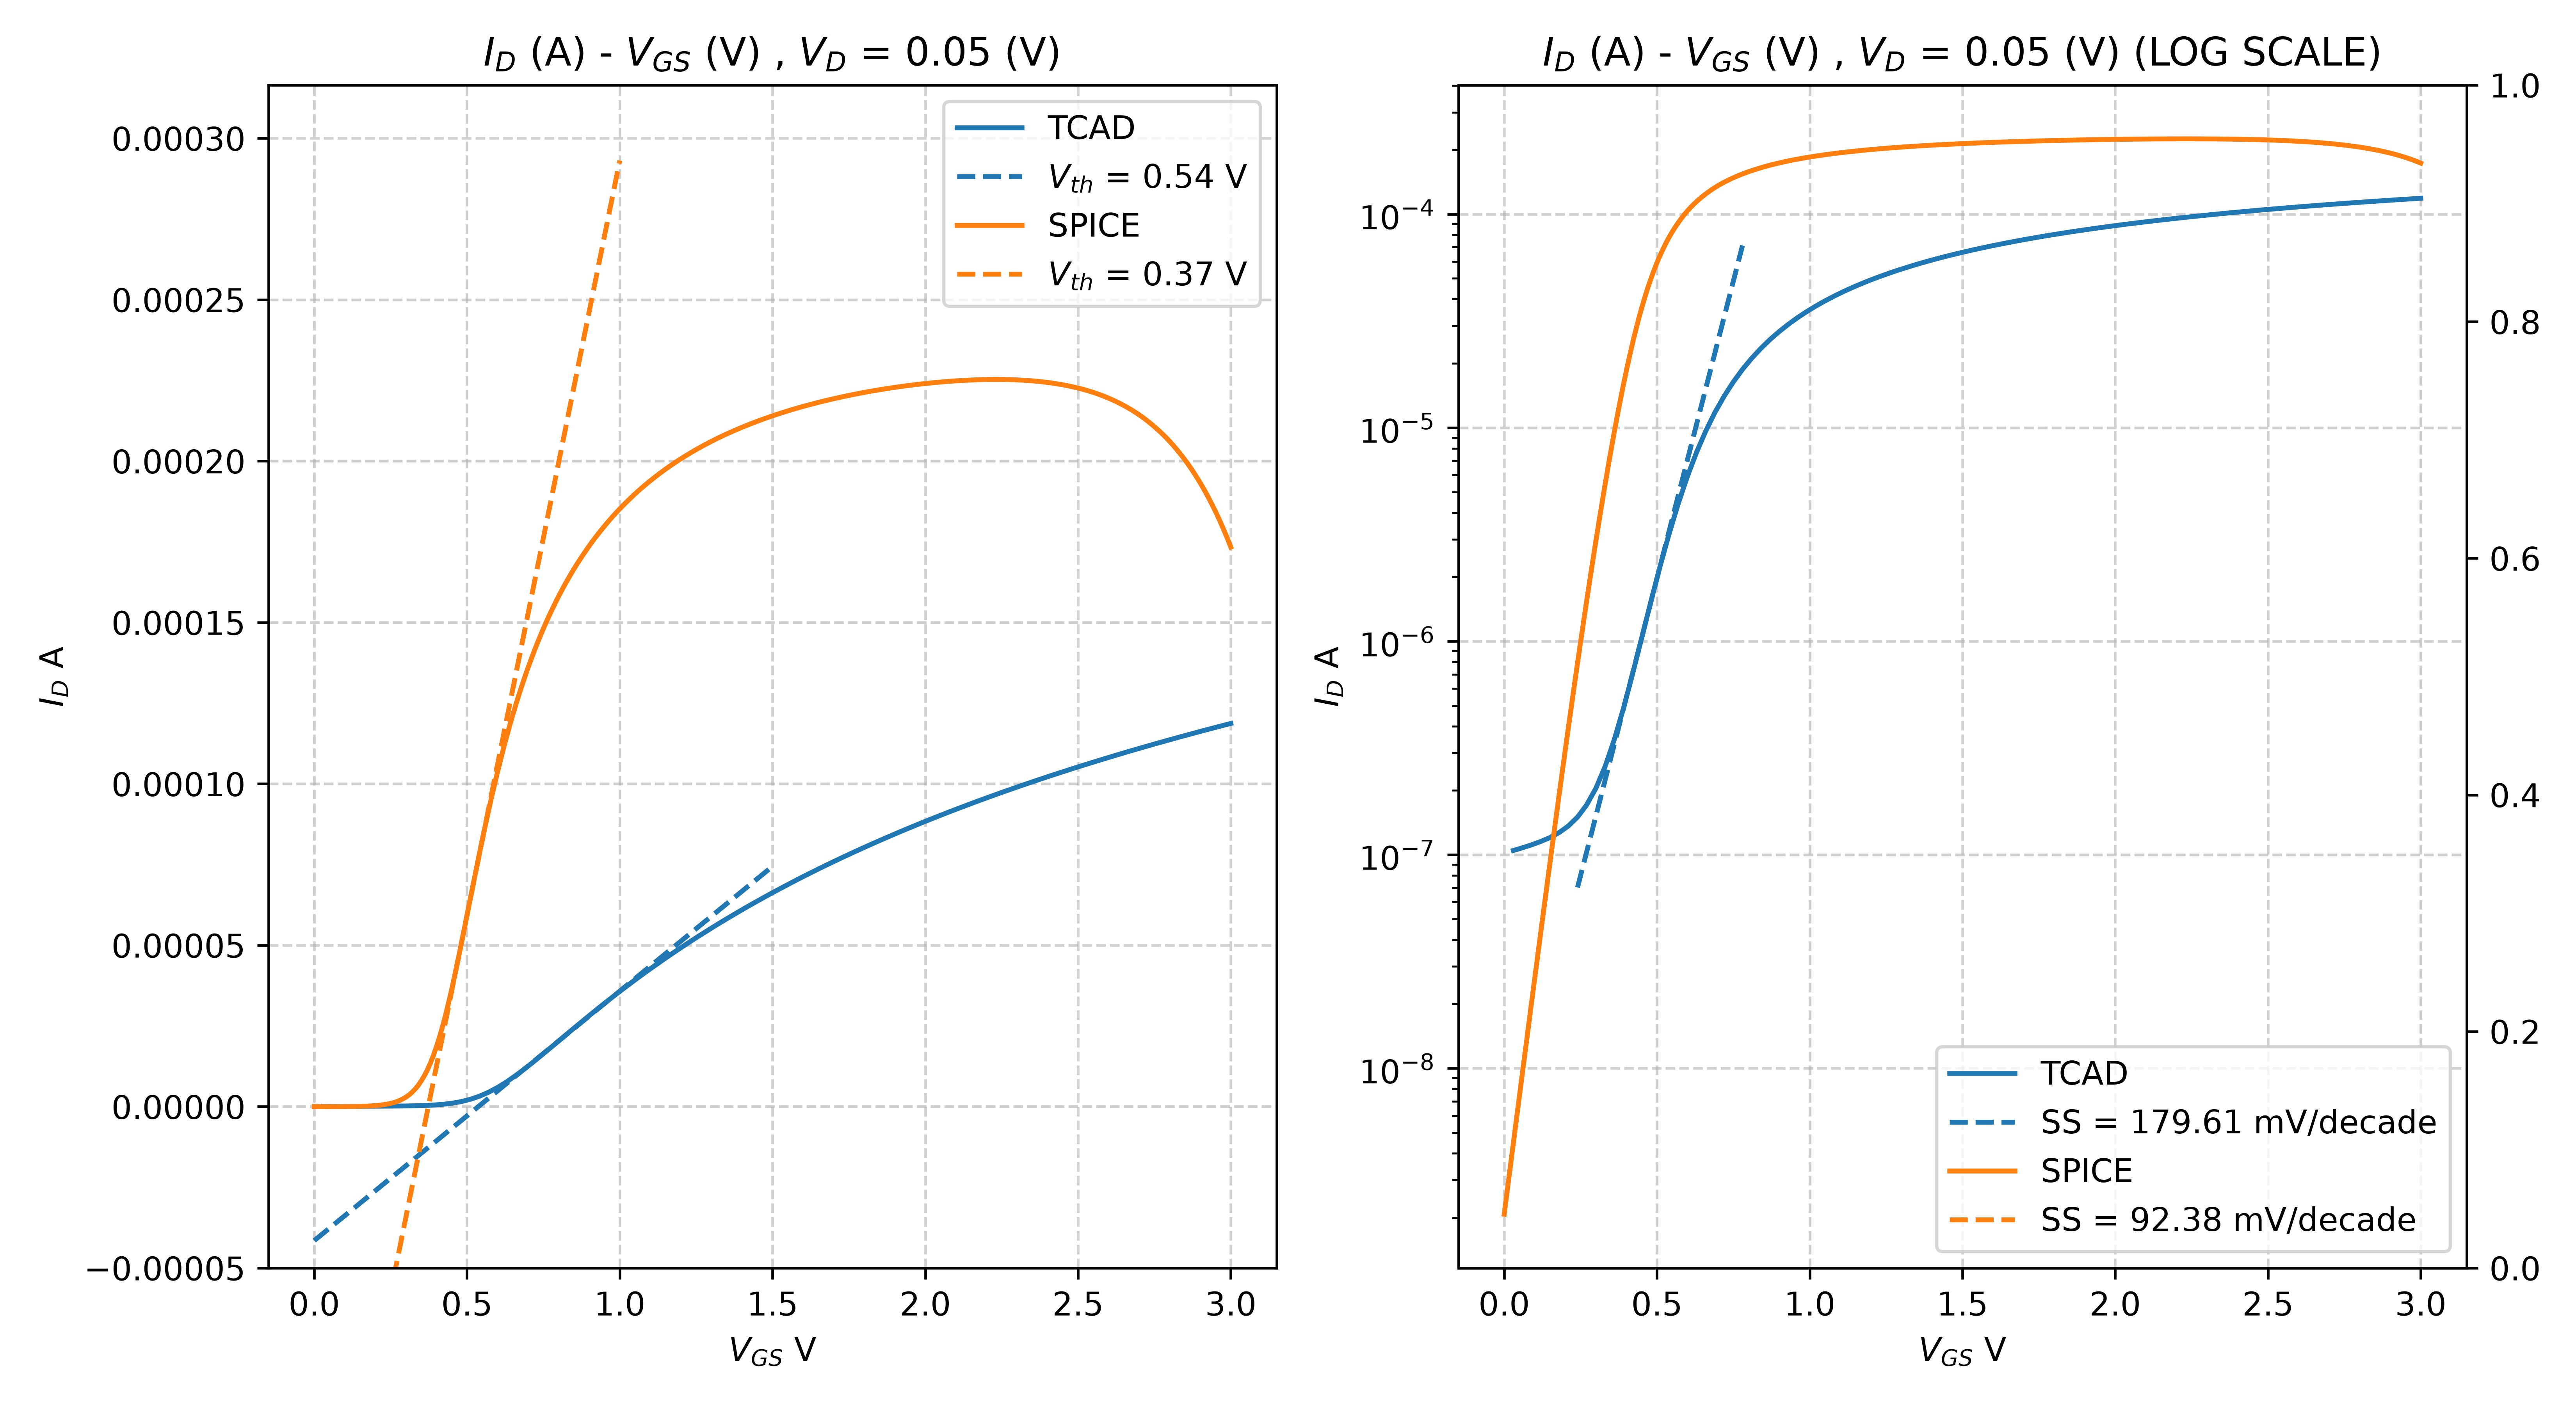
\includegraphics[width=\textwidth]{s2.png}
\vspace{-0.5em}
\captionof{figure}{$I_D$--$V_G$ at $V_{DS}=50$~mV and $1.1$~V ($L=65$~nm).}

\begin{table}[H]\centering
\begin{tabular}{@{}lcccc@{}}\toprule
 Parameter & Extracted (SPICE) & Table 5.1 (TCAD)\\\midrule
$V_{TH}$ (V)                    & 0.37 & 0.54 \\
$I_{ON}$ ($\mu$A/$\mu$m)   ($V_G$ = 1.1 v)     & 193.9& 41.32 \\
$I_{OFF}$ (nA/$\mu$m)           & 2.07 & 104.66 \\
SS (mV/dec)                     & 92.38& 179.61 \\\bottomrule
\end{tabular}
\caption{Comparison of extracted parameters, \(V_D = 0.05v\)}
\end{table}
\begin{observations}\todo{Agreement / mismatch with the table; reason for $V_{TH}$ shift between the two $V_{DS}$ (DIBL).}\vspace{1.5cm}\end{observations}
\begin{conclusion}\todo{Key takeaway.}\vspace{1cm}\end{conclusion}
\clearpage

% ============================================================
\section{S3 -- Output Characteristics}
\circuit{s3-circuit.png}{LTspice testbench for the $I_D$--$V_D$ family.}{.dc vd 0 1.5 0.01 \\
.step param v list 0.3 0.6 0.9 1.5}

\onefig{s3.png}{0.8\textwidth}{7.5cm}{$I_D$--$V_D$ family at $V_{GS}=0.3,\,0.6,\,0.9,\,1.5$~V.}
\onefig{gd_vs_vds.png}{0.8\textwidth}{6cm}{$g_{ds}$ (via \texttt{np.gradient}) versus $V_{DS}$; saturation region marked at $V_{GS}=1.5$~V.}

\begin{table}[H]\centering
\begin{tabular}{@{}lcc@{}}\toprule
Quantity (at $V_{GS}=1.5$~V, saturation) & SPICE & TCAD \\\midrule
$V_{DS}$ range used for $g_{ds}$ (V) & 1.17 - 2 &  1.17 - 2\\
$g_{ds}$ ($\mu$S/$\mu$m) & 312.16& 329.87\\
$r_o = 1/g_{ds}$ (k$\Omega\cdot\mu$m) & 3.20 & 3.03\\\bottomrule
\end{tabular}
\caption{Output conductance and resistance.}
\end{table}
\begin{observations}\todo{Linear vs.\ saturation region, finite output resistance, CLM / DIBL / velocity saturation.}\vspace{1.5cm}\end{observations}
\begin{conclusion}\todo{Key takeaway.}\vspace{1cm}\end{conclusion}
\clearpage

% ============================================================
\section{S4 -- Physics Check}
\circuit{s4-circuit.png}{LTspice testbench for the model-parameter checks (\textit{UA}, \textit{UB}, \textit{VSAT}).}{.dc vg 0 3 0.01}

\onefig{s4.png}{0.85\textwidth}{8cm}{$I_D$--$V_G$ overlay: nominal, $UA=UB=0$, and $VSAT\times100$. (Log axis recommended; add a linear inset if useful.)}

% \begin{table}[H]\centering
% \begin{tabular}{@{}lccc@{}}\toprule
% Case & $V_{TH}$ (V) & $I_{ON}$ ($\mu$A/$\mu$m) & $I_{OFF}$ (nA/$\mu$m)\\\midrule
% Nominal                 & & & \\
% $UA=UB=0$               & & & \\
% $VSAT\times100$         & & & \\\bottomrule
% \end{tabular}
% \caption{Effect of switching off individual physical models.}
% \end{table}

\begin{physics}
\textbf{$UA=UB=0$ $\leftrightarrow$ TCAD \emph{Enormal} (mobility degradation) model:}
\todo{explain vertical-field mobility degradation, surface-roughness scattering, effect on $I_{ON}$.}\vspace{1.2cm}

\textbf{$VSAT\times100$ $\leftrightarrow$ TCAD \emph{HighFieldSaturation} model:}
\todo{explain removal of velocity saturation, effect on $I_{ON}$ and saturation behaviour.}\vspace{1.2cm}
\end{physics}
\begin{conclusion}\todo{Which effect limits $I_{ON}$ most in a 65\,nm device?}\vspace{1cm}\end{conclusion}
\clearpage

% ============================================================
\section{S5 -- Parametric Variation}
\circuit{s5-circuit1.png}{Circuit of $I_D$-$V_G$}{.dc vg 0 1.5 0.01}
\circuit{s5-circuit2.png}{Circuit of $I_D$-$V_D$}{.dc vd 0 1.5 0.01}


\noindent Each experiment varies one parameter around its nominal value. $I_D$--$V_G$ is simulated at $V_{DS}=0.4$~V and $I_D$--$V_D$ at $V_{GS}=1.1$~V.

\subsection*{Summary of Experiments}
\begin{table}[H]\centering\small
\begin{tabular}{@{}clll@{}}\toprule
Exp. & Parameter & Low / Nominal / High & Unit\\\midrule
1  & VTH0  & 0.30 / 0.423 / 0.55 & V\\
2  & TOXE  & 1.5 / 1.85 / 2.5 & nm\\
3  & L (drawn) & 55 / 65 / 100 & nm\\
4  & XL    & $-35$ / $-30$ / $-15$ & nm\\
5  & LINT  & 2 / 5.25 / 8 & nm\\
6  & W (drawn) & 0.5 / 1 / 2 & $\mu$m\\
7  & WINT  & 0 / 5 / 40 & nm\\
8  & NDEP  & $1.5\times10^{18}$ / $2.54\times10^{18}$ / $4\times10^{18}$ & cm$^{-3}$\\
9  & NSD   & $5\times10^{19}$ / $2\times10^{20}$ / $5\times10^{20}$ & cm$^{-3}$\\
10 & XJ    & 10 / 19.6 / 30 & nm\\
11 & NGATE & $1\times10^{19}$ / $2\times10^{20}$ / $1\times10^{21}$ & cm$^{-3}$\\
12 & U0    & 300 / 491 / 700 & cm$^2$/V$\cdot$s\\
13 & VSAT  & $0.8\times10^{7}$ / $1.24\times10^{7}$ / $2\times10^{7}$ & cm/s\\
14 & RDSW  & 50 / 165 / 400 & $\Omega\cdot\mu$m\\\bottomrule
\end{tabular}
\caption{Parameters varied in S5 (the handout text says ``1 to 13'' but lists 14 rows).}
\end{table}
\clearpage

\expblock{1}{VTH0}{0.30 / 0.423 / 0.55~V}{VTH0}
\expblock{2}{TOXE}{1.5 / 1.85 / 2.5~nm}{TOXE}
\expblock{3}{L (drawn)}{55 / 65 / 100~nm}{L_drawn}
\expblock{4}{XL}{$-35$ / $-30$ / $-15$~nm}{XL}
\expblock{5}{LINT}{2 / 5.25 / 8~nm}{LINT}
\expblock{6}{W (drawn)}{0.5 / 1 / 2~$\mu$m}{W_drawn}
\expblock{7}{WINT}{0 / 5 / 40~nm}{WINT}
\expblock{8}{NDEP}{$1.5\times10^{18}$ / $2.54\times10^{18}$ / $4\times10^{18}$~cm$^{-3}$}{NDEP}
\expblock{9}{NSD}{$5\times10^{19}$ / $2\times10^{20}$ / $5\times10^{20}$~cm$^{-3}$}{NSD}
\expblock{10}{XJ}{10 / 19.6 / 30~nm}{XJ}
\expblock{11}{NGATE}{$1\times10^{19}$ / $2\times10^{20}$ / $1\times10^{21}$~cm$^{-3}$}{NGATE}
\expblock{12}{U0}{300 / 491 / 700~cm$^2$/V$\cdot$s}{U0}
\expblock{13}{VSAT}{$0.8\times10^{7}$ / $1.24\times10^{7}$ / $2\times10^{7}$~cm/s}{VSAT}
\expblock{14}{RDSW}{50 / 165 / 400~$\Omega\cdot\mu$m}{RDSW}

\subsection{Overall Summary of S5}
\begin{table}[H]\centering\small
\begin{tabular}{@{}clcccl@{}}\toprule
Exp. & Parameter & $V_{TH}$ & $I_{ON}$ & $I_{OFF}$ & Matches expectation? (Y/N, reason)\\\midrule
1 & VTH0 & & & & \\
2 & TOXE & & & & \\
3 & L & & & & \\
4 & XL & & & & \\
5 & LINT & & & & \\
6 & W & & & & \\
7 & WINT & & & & \\
8 & NDEP & & & & \\
9 & NSD & & & & \\
10 & XJ & & & & \\
11 & NGATE & & & & \\
12 & U0 & & & & \\
13 & VSAT & & & & \\
14 & RDSW & & & & \\\bottomrule
\end{tabular}
\caption{Trend summary ($\uparrow$, $\downarrow$, $\approx$ as the parameter increases).}
\end{table}
\begin{conclusion}\todo{Which parameters dominate $V_{TH}$, $I_{ON}$, $I_{OFF}$? Which behave unexpectedly in SPICE and why?}\vspace{1.5cm}\end{conclusion}
\clearpage

% ============================================================
\section{S6 -- Approximate Match to TCAD}
\circuit{s6-circuit.png}{LTspice testbench used for the TCAD comparison.}{* .dc Vg ... / .dc Vd ... (paste here)}

\twofig{s6-idvg-match.png}{$I_D$--$V_G$, $V_{DS}=0.4$~V (linear)}{s6-idvd-match.png}{$I_D$--$V_D$, $V_{GS}=0.9$~V (linear)}{}{6.5cm}
\vspace{-0.5em}
\captionof{figure}{TCAD (markers) versus tuned SPICE (lines).}

\begin{table}[H]\centering
\begin{tabular}{@{}lccl@{}}\toprule
Parameter & PTM value & My value & Reason for change\\\midrule
 & & & \\
 & & & \\
 & & & \\
 & & & \\
 & & & \\
 & & & \\\bottomrule
\end{tabular}
\caption{Parameters modified in \texttt{nfit}.}
\end{table}

\begin{table}[H]\centering
\begin{tabular}{@{}lccc@{}}\toprule
Metric & TCAD & SPICE (tuned) & Error (\%)\\\midrule
$V_{TH}$ & & & \\
$I_{ON}$ & & & \\
$I_{OFF}$ & & & \\
$r_o$ & & & \\\bottomrule
\end{tabular}
\caption{Quality of match.}
\end{table}
\begin{observations}\todo{Where the match is good, where it fails (e.g.\ subthreshold, saturation slope) and why a perfect match is not possible.}\vspace{1.5cm}\end{observations}
\clearpage

% ============================================================
\section{S7 -- CMOS Inverter}
\subsection{Circuit and Parameters}
\begin{figure}[H]\centering
\gfx{s7-circuit.png}{0.35\textwidth}{6cm}
\caption{LTspice schematic of the CMOS inverter.}
\end{figure}
\begin{table}[H]\centering
\begin{tabular}{@{}lcc@{}}\toprule
Parameter & nMOS & pMOS\\\midrule
$L$   & 65 nm & 65 nm\\
$W$   & 1 $\mu$m & 2 $\mu$m\\
$V_{DD}$ & 1.1 V & 1.1 V\\\bottomrule
\end{tabular}
\end{table}

\subsection{Voltage Transfer Characteristic}
\onefig{s7.png}{0.75\textwidth}{7cm}{$V_{out}$ versus $V_{in}$ ($0\to V_{DD}$); mark $V_{OH}$, $V_{OL}$, $V_M$ and the gain region.}

\begin{table}[H]\centering
\begin{tabular}{@{}lc@{}}\toprule
Quantity & Value\\\midrule
$V_{OH}$ (V) & \\
$V_{OL}$ (V) & \\
Switching threshold $V_M$ (V) & \\
Max.\ gain $|dV_{out}/dV_{in}|$ & \\\bottomrule
\end{tabular}
\caption{Inverter metrics from the VTC.}
\end{table}
\begin{physics}\todo{Explain operation in each region (NMOS off/PMOS on, both in saturation, NMOS on/PMOS off) and why the circuit is called an ``inverter''.}\vspace{2cm}\end{physics}
\begin{conclusion}\todo{Key takeaway, effect of the $W_p/W_n=2$ ratio on $V_M$.}\vspace{1cm}\end{conclusion}
\clearpage

% ============================================================
\section{S8 -- GitHub Repository}
\begin{itemize}
  \item Repository name: \texttt{LTSPICE}
  \item URL: \blank[9cm]
\end{itemize}
\begin{table}[H]\centering
\begin{tabular}{@{}ll@{}}\toprule
Python script & Purpose\\\midrule
\texttt{s2\_transfer.py} & S2: $I_D$--$V_G$ plots and extraction\\
\texttt{s3\_output.py}   & S3: $I_D$--$V_D$ family, $g_{ds}$, $r_o$\\
\texttt{s4\_physics.py}  & S4: model overlay\\
\texttt{s5\_param.py}    & S5: parametric sweeps\\
\texttt{s6\_fit.py}      & S6: TCAD vs SPICE overlay\\
\texttt{s7\_inverter.py} & S7: VTC plot\\\bottomrule
\end{tabular}
\caption{Scripts committed to the repository (rename to match yours).}
\end{table}

\section{Overall Conclusions}
\begin{enumerate}
  \item \todo{Conclusion 1}
  \item \todo{Conclusion 2}
  \item \todo{Conclusion 3}
  \item \todo{Conclusion 4}
\end{enumerate}
\vspace{3cm}

\section*{References}
\addcontentsline{toc}{section}{References}
\begin{enumerate}
  \item EC2L104 Course Handout: \emph{A Beginner's Manual to SPICE Modelling in LTspice}.
  \item PTM -- Predictive Technology Model, 65\,nm BSIM4 model card.
  \item \todo{Any additional references.}
\end{enumerate}

\appendix
\section{Appendix: Python Code Listings}
\begin{lstlisting}[language=Python]
# paste key code snippets here (full code is in the GitHub repo)
\end{lstlisting}

\section{Appendix: Full Model Card}
\begin{lstlisting}
* paste the nfit model card here
\end{lstlisting}

\end{document}